% ===========================================================================
\section{A resolução: quanto custa ver}\label{sec:resolucao}
% ===========================================================================

Um pico é um objeto de largura finita, e a largura é determinada pela janela de
observação. Nesta seção tornamos essa afirmação quantitativa, obtemos a lei de
escala do desenho de um bloco e o custo de ver um único primo.

\subsection{O critério de Rayleigh}

Sejam dois tons de frequências $\nu_1<\nu_2$ (em radianos) e amplitudes $a_1,a_2$,
observados em $[0,T]$. O coeficiente de um tom na frequência do outro é regido
pelo núcleo de Dirichlet.

\begin{lema}\label{lema:kernel}
Com $\delta=\nu_2-\nu_1>0$ e $T>0$,
\[
  \left|\int_0^T\cos(\nu_2 t)\,e^{-i\nu_1 t}\,dt\right|
  \;=\;
  \left|\frac{\sin(\delta T/2)}{\delta/2}\right|\cdot\bigl(1+O((T\nu_1)^{-1})\bigr).
\]
Em particular o coeficiente se anula quando $\delta T/(2\pi)\in\Z\setminus\{0\}$ e
vale $\approx T/2$ quando $\delta T\ll1$.
\end{lema}

\begin{proof}
Escreva $2\cos(\nu_2t)=e^{i\nu_2t}+e^{-i\nu_2t}$ e integre $e^{i(\nu_2-\nu_1)t}$ e
$e^{-i(\nu_2+\nu_1)t}$; a primeira integral vale
$\bigl|e^{i\delta T}-1\bigr|/\delta=2|\sin(\delta T/2)|/\delta$, a segunda é
$O(1/(\nu_1+\nu_2))$.
\end{proof}

O Lema~\ref{lema:kernel} diz que a largura do lóbulo principal de um pico, medida
entre os dois zeros vizinhos, é $2\pi/T$ em radianos, isto é, $1/T$ em ciclos.
Dois tons são \emph{resolvidos} quando o pico de um não cai dentro do lóbulo
principal do outro, o que dá o critério clássico.

\begin{lema}[Rayleigh]\label{lema:rayleigh}
Para que dois tons de frequências $\freq{q_1}<\freq{q_2}$ apareçam como picos
distintos numa janela de comprimento $T$, é necessário
\[
  T \;>\; \frac{2\pi}{\log(q_2/q_1)} \;=\; \frac{1}{\freq{q_2}-\freq{q_1}} .
\]
\end{lema}

\begin{proof}
O primeiro zero do núcleo do Lema~\ref{lema:kernel} ocorre em
$\delta T=2\pi$, isto é, $T=1/(\freq{q_2}-\freq{q_1})$.
\end{proof}

\subsection{O par gargalo e a lei de escala}

Pelo Lema~\ref{lema:rayleigh}, o comprimento de janela exigido por um par é
$2\pi/\log(q_2/q_1)$, tanto maior quanto menor for o \emph{gap relativo}
$\log(q_2/q_1)=\log(1+g/q_1)$ do par. Para primos consecutivos, $g\ge2$, e a
igualdade $g=2$ caracteriza os pares de gêmeos.

\begin{definicao}\label{def:gargalo}
Para um conjunto finito $\Seed$ de primos com $\#\Seed\ge2$, o \emph{par gargalo} é
o par de primos consecutivos $q_1<q_2$ de $\Seed$ que maximiza
$2\pi/\log(q_2/q_1)$, e
\[
  \tau(\Seed) \;=\; \frac{2\pi}{\max\log(q_2/q_1)}
\]
é a \emph{janela exigida} por $\Seed$.
\end{definicao}

\begin{teorema}[lei de escala]\label{teo:custo}
Seja $Q_k=\max \Seed_k$ (o maior primo abaixo de $2^k$) e $m_k=\#\Seed_k$. Então
\[
  \frac{2\pi}{\log\bigl(1+2/(Q_k-2)\bigr)}
  \;\le\; \tau(\Seed_k) \;\le\; 2\pi\,(m_k-1),
\]
e, como $m_k\asymp 2^k/k$ e $Q_k\asymp 2^k$, vale
$\tau(\Seed_k)=\Theta(2^k/k)$ com constantes explícitas.
\end{teorema}

\begin{proof}
\emph{Cota superior.} Seja $q_1<q_2$ um par qualquer de $\Seed_k$, com gap
$g=q_2-q_1\ge2$. Como $q_1\le Q_k-2$, temos $g/q_1\ge 2/(Q_k-2)$, donde
$\log(q_2/q_1)=\log(1+g/q_1)\ge\log(1+2/(Q_k-2))$ e portanto
$2\pi/\log(q_2/q_1)\le 2\pi/\log(1+2/(Q_k-2))$.

\emph{Cota inferior.} Os $m_k$ elementos de $\Seed_k$ estão todos em
$[2,Q_k-1]$, um intervalo de comprimento $Q_k-2$; logo algum par de consecutivos
tem gap $g\le (Q_k-2)/(m_k-1)$. Para esse par,
$\log(q_2/q_1)=\log(1+g/q_1)\le g/q_1\le 1/(m_k-1)$, e assim
$2\pi/\log(q_2/q_1)\ge 2\pi(m_k-1)$.

\emph{Assintótica.} Pelo teorema dos números primos $m_k\sim 2^k/(k\log2)$, e
$2^{k-1}<Q_k<2^k$; substituindo nas duas cotas obtém-se o mesmo expoente.
\end{proof}

Em palavras: a janela necessária para desenhar um bloco cresce como $2^k/k$, isto
é, essencialmente como o próprio bloco dividido por um fator logarítmico. A
Figura~\ref{fig:lei} mostra as duas pontas do Teorema~\ref{teo:custo} para
$k=4,\dots,22$: a curva medida cresce exponencialmente e, o que é mais preciso,
coincide com $\pi q_{\text{gêmeo}}$, onde $q_{\text{gêmeo}}$ é o maior elemento de
um par de gêmeos da semente.

\begin{figure}[htbp]
\centering
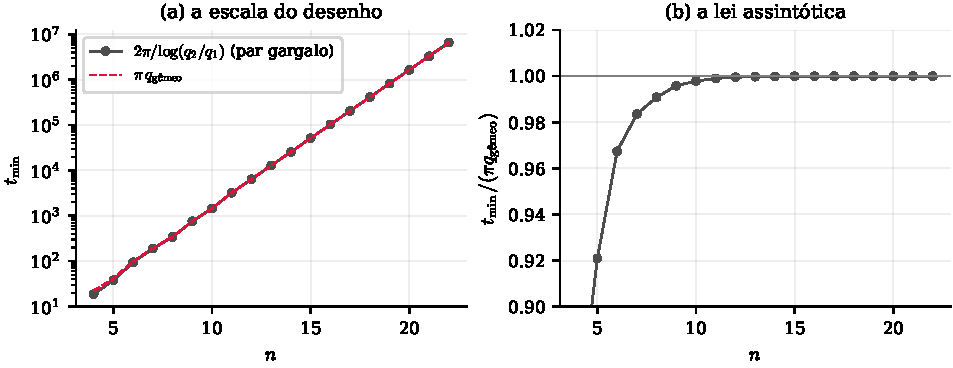
\includegraphics[width=0.95\textwidth]{figuras/f3_lei.pdf}
\caption{(a) A janela exigida pelo par gargalo de $\Seed_k$, em escala
logarítmica; a curva é indistinguível de $\pi q_{\text{gêmeo}}$. (b) A razão entre
os dois tende a $1$: o erro relativo já é $10^{-3}$ em $n=9$.}
\label{fig:lei}
\end{figure}

\begin{table}[htbp]
\centering
\footnotesize
\begin{tabular}{rrrrr}
\toprule
$n$ & par gargalo & janela exigida & $\pi\,q_{\text{gêmeo}}$ & razão \\
\midrule
6  & $(29,\,31)$        & $94{,}2$      & $97{,}4$      & 0,967 \\
8  & $(107,\,109)$      & $339{,}3$     & $342{,}4$     & 0,991 \\
10 & $(461,\,463)$      & $1\,451{,}4$  & $1\,454{,}6$  & 0,998 \\
12 & $(2\,027,\,2\,029)$& $6\,371{,}1$  & $6\,374{,}3$  & 0,9995 \\
14 & $(8\,087,\,8\,089)$& $25\,409{,}2$ & $25\,412{,}3$ & 0,9999 \\
\bottomrule
\end{tabular}
\caption{O par gargalo é sempre um par de gêmeos nas escalas verificadas, e a
janela exigida coincide com $\pi q_{\text{gêmeo}}$ no limite.}
\label{tab:lei}
\end{table}

\subsection{O custo de ver um primo}

O Teorema~\ref{teo:custo} é sobre um bloco inteiro. Há uma versão local, que é a
que responde à pergunta ``quanto custa verificar que $q$ é primo olhando o
espectro?''.

\begin{corolario}[custo local]\label{cor:local}
Seja $q\ge5$ primo e considere o sinal $R$ definido em \eqref{eq:Rprimo}, com
$N\ge q$. Para decidir, com margem constante, se o tom de frequência $\nfreq q$
está presente, é necessário uma janela $T=\Omega(q)$; e $T$ proporcional a $q$
com constante adequada é suficiente.
\end{corolario}

\begin{proof}
A prova é a Proposição~\ref{prop:gemeo} da Seção~\ref{sec:assinatura}, que
quantifica o resíduo: na ausência do tom — isto é, se $q$ não está na soma — a
amplitude relativa em $\nfreq q$ é $O(q/T)$, enquanto a presença do tom dá
$1+O(\sqrt q/T)$. Separar os dois com margem fixa exige $T\gg q$, e $T$
proporcional a $q$ com constante adequada basta.
\end{proof}

O contraste com a aritmética é o ponto. A divisão de tentativas decide a
primalidade de $q$ em $O(\sqrt q)$ operações, sem sinal e sem janela. Ver $q$ no
espectro custa uma janela de comprimento proporcional a $q$. O fator entre as duas
escalas é $\sqrt q$: é o preço, em resolução, de representar a irredutibilidade
como uma propriedade de frequência em vez de uma propriedade de divisibilidade.

Isso não é um defeito da construção — é uma medida. O dicionário da
Seção~\ref{sec:dicionario} é fiel, e a fidelidade tem este custo: para separar
$\nfreq q$ do tom do primo vizinho, cuja distância relativa é $\approx 2/q$, a
janela precisa ser da ordem de $q$.

\subsection{A janela de leitura}

Na prática, para localizar um pico mede-se o máximo da amplitude em uma faixa de
$\pm W$ células em torno da frequência procurada. Essa escolha introduz um segundo
parâmetro, que não tem nada a ver com $T$ e que pode arruinar a leitura.

\begin{proposicao}[janela de leitura]\label{prop:janela}
Seja $q\ge5$ primo e $\delta=\log\bigl(q/(q-2)\bigr)$ a distância entre as
frequências de $q$ e de $q-2$. Para que a faixa de $\pm W$ células em torno de
$\freq q$ não contenha o lóbulo principal do pico de $q-2$, é necessário
\[
  2W+1 \;<\; \frac{T\,\delta}{2\pi} \;\approx\; \frac{T}{\pi q} .
\]
\end{proposicao}

\begin{proof}
É o Lema~\ref{lema:rayleigh} aplicado ao par $(q-2,q)$, com a largura $2W+1$ da
faixa no lugar de uma célula, e $\delta=\log(1+2/(q-2))\ge 2/q$.
\end{proof}

A Proposição~\ref{prop:janela} explica por que medidas com a mesma janela $T$
podem discordar: se a faixa de leitura for larga em relação ao gap, o máximo lido
em $\freq q$ é o pico do vizinho. Para $q\approx300$ e $T=6500$, o lado direito
vale $6{,}9$ células; uma leitura com $W=2$ é segura, uma com $W=10$ não é. A
Tabela~\ref{tab:janela} registra o efeito.

\begin{table}[htbp]
\centering
\small
\begin{tabular}{rrrrr}
\toprule
$T$ & $W=0$ & $W=2$ & $W=10$ & $T/(\pi q_{\max})$ \\
\midrule
$1\,500$ & $100\%$ & $77\%$ & $42\%$ & $1{,}6$ \\
$6\,500$ & $100\%$ & $100\%$ & $77\%$ & $6{,}9$ \\
\bottomrule
\end{tabular}
\caption{Acurácia da separação entre pares gêmeos e mistos
(Seção~\ref{sec:assinatura}) em função da meia-largura $W$ da faixa de leitura,
para $N=300$. A separação sobrevive enquanto $2W+1<T/(\pi q_{\max})$.}
\label{tab:janela}
\end{table}
